\visHeader
\subsection{The Enterprise Architect Control Panel (Visual) }

\hypertarget{validation vis}{Our} EA extension provides rudimentary support for validating both the static semantics (Ecore) and dynamic semantics (SDM) of
metamodels. Validation results are displayed and, in some cases, even ``quick fixes'' to automatically solve the problems are offered. Our validation framework
is still work in progress so if you find an error that is not/wrongly detected, feel free to send us a brief description of the issue.

\begin{enumerate}
\item[$\blacktriangleright$] To make the validation output window visible in EA, choose ``Extensions/\-Add-In Windows''. This should display a new output window
as depicted in Fig.~\ref{fig:validation_output}. This control panel also contains shortcuts for all the functionality available via the extensions file menu.
Many users prefer this, and so we hope you'll find it useful.

\begin{figure}[htbp]
	\centering
  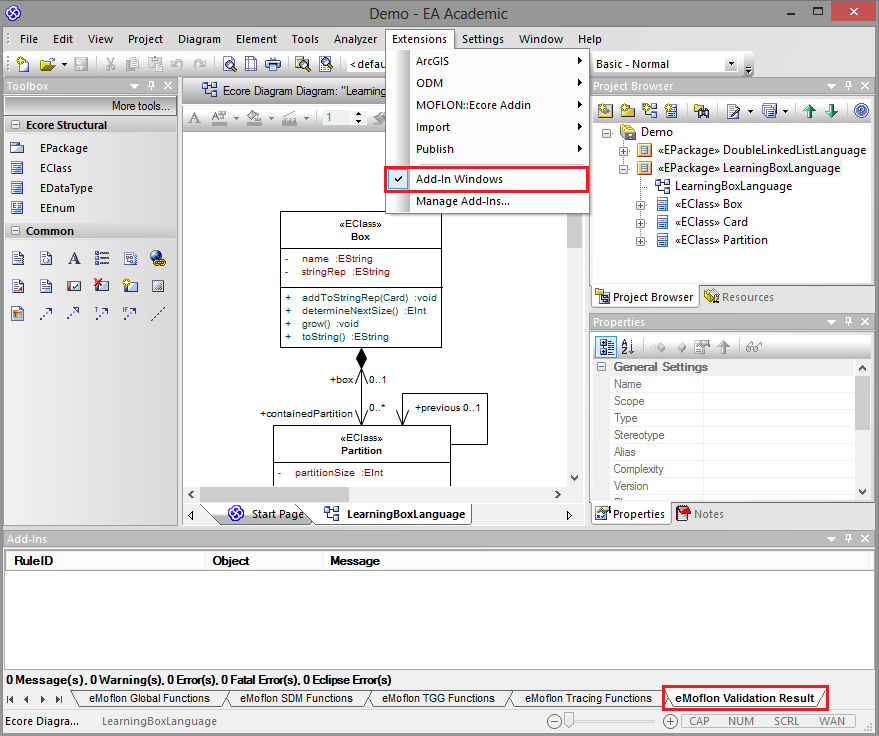
\includegraphics[width=0.7\textwidth]{ea_activateAddInWindow}
	\caption{Activating the validation output window}
	\label{fig:validation_output}
\end{figure}
\FloatBarrier

\item[$\blacktriangleright$] To start the validation choose ``Extensions/\-MOFLON::Ecore Addin/\-Validate all'' in EA (Fig.~\ref{fig:validation_menu}).
If you haven't made any mistakes while modelling your \texttt{LearningBoxLanguage} in the previous sections, the output should still resemble
Fig.~\ref{fig:validation_output}, indicating that your metamodels are free of errors.

\begin{figure}[htbp]
	\centering
  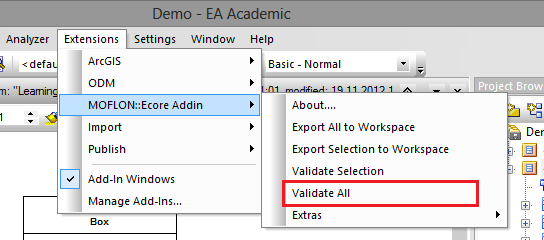
\includegraphics[width=0.6\textwidth]{ea_startValidation}
	\caption{Starting the validation}
	\label{fig:validation_menu}
\end{figure}
\FloatBarrier
\end{enumerate}


Why don't we try to get familiar with our validation and quick fix features? Let's add two small modelling errors in \texttt{LearningBoxLanguage}.

\begin{enumerate}
\item[$\blacktriangleright$] Create a new class in the \texttt{Learning\-Box\-Language} diagram. You can retain the default name \texttt{EClass1}. Let's assume,
you wish to delete this class from your metamodel.

\item[$\blacktriangleright$] Select it (\texttt{EClass1}) in the diagram and press the \texttt{Delete} button. Note that \texttt{EClass1} still exists in the
project browser (and thus in your metamodel). You should have one new \texttt{Information} message in the validation output
(Fig.~\ref{fig:validation_information}).

\begin{figure}[htbp]
	\centering
  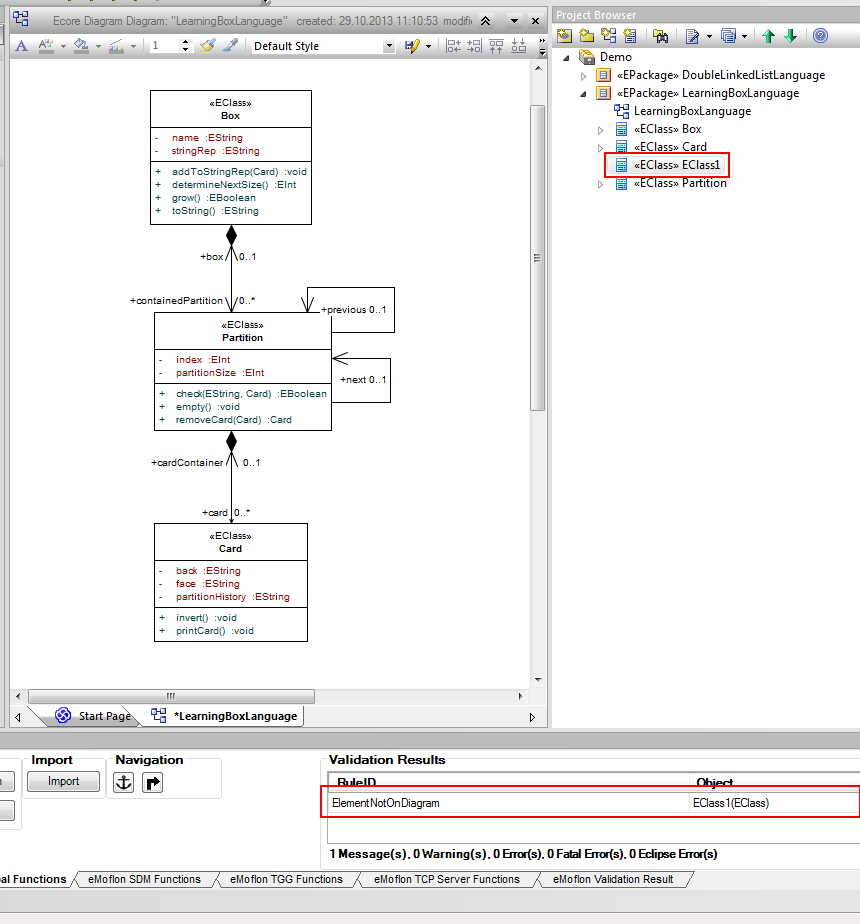
\includegraphics[width=0.6\textwidth]{EA_validationDeleteElement}
	\caption{Validation information error: element still exists}
	\label{fig:validation_information}
\end{figure}

\pagebreak

The message informs you that \texttt{EClass1} is not on any diagram, and seeing as it is still in the model, that this could be a mistake. Just pressing the
\texttt{Delete} button is not the proper way of removing \texttt{EClass1} from the metamodel. It only removes it from the current diagram! Deleting elements
properly and other EA specific aspects are discussed in detail in \texttt{Part VI: Micellaneous}.


\item[$\blacktriangleright$] To navigate to the problematic element click once on the information message in the output window. EA should navigate automatically
to \texttt{EClass1} and highlight it in the project browser.

\item[$\blacktriangleright$] To check to see if there are any quick fixes available, double click the information message to invoke the ``QuickFix'' dialogue.
In this case, there is one quick fix which suggests to simply delete the element from the model (Fig.~\ref{fig:quick-fix1}) as this is probably what was
intended.

\begin{figure}[htbp]
	\centering
  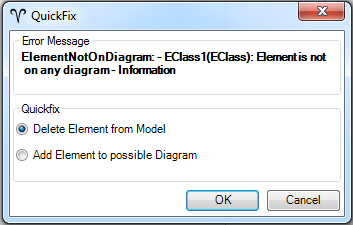
\includegraphics[width=0.55\textwidth]{ea_quickFixElements}
	\caption{Quick fix for elements that are not on any diagram}
	\label{fig:quick-fix1}
\end{figure}
\FloatBarrier

\item[$\blacktriangleright$] Click \texttt{OK} and \texttt{EClass1} will be deleted correctly from your model\footnote{If it wasn't, you can manually delete the
class by going to the Project Browser, and selecting \texttt{Delete <<EClass>> EClass1}. Such is the proper way to delete elements from your model.}. Your
metamodel should now be error-free again as indicated by the validation output window.

\item[$\blacktriangleright$] To make an error that leads to a more critical message than ``information,'' double click the navigable reference end
\texttt{previous} of the class \texttt{Partition}, and delete its role name as depicted in Fig.~\ref{fig:delete-role-name}. Affirm with \texttt{OK}.

\begin{figure}[htbp]
    \centering
  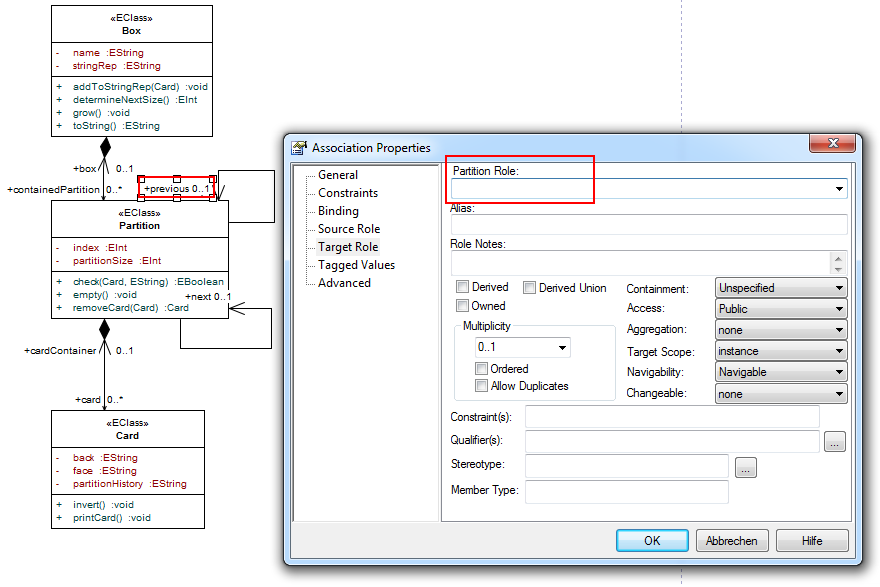
\includegraphics[width=0.85\textwidth]{EA_validationDeleteRoleName}
    \caption{Deleting a navigable role name of a reference}
    \label{fig:delete-role-name}
\end{figure}


\begin{figure}[htbp]
	\centering
  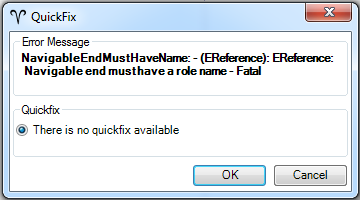
\includegraphics[width=0.6\textwidth]{EA_quickFixFatal}
	\caption{Fatal error after deleting a navigable role name}
	\label{fig:fatal-error}
\end{figure}

You should now see a new \texttt{Fatal Error} in the validation output, stating that a navigable end \emph{must} have a role name. Double click the error to
view the quick fix menu (Fig.~\ref{fig:fatal-error}). As navigable references are mapped to data members in a Java class, omitting the name of a navigable
reference makes code generation impossible (data members (i.e., class variables) must have a name).

\item[$\blacktriangleright$] Given there are no automatic solutions, correct your metamodel manually by setting the name of the navigable reference back to
\texttt{previous}.

\item[$\blacktriangleright$] Ensure that your metamodel closely resembles Fig.~\ref{fig:metamodel_complete} again, and that there are no error messages before
you proceed with the rest of this handbook.
\end{enumerate}

As you may have already noticed, we distinguish between five different types of validation messages:
\begin{description}
  \item[Information:]~\\
  This is only a hint for the user and can be safely ignored if you know what you're doing.
  Export and code generation should be possible, but certain naming/modelling conventions are violated, or a problematic situation has been detected.
  
  \item[Warning:]~\\ Export and code generation is possible, but only with defaults and automatic corrections applied by the code generator.
  As this might not be what the user wants, such cases are flagged as warnings (e.g., omitting the multiplicity at references which is automatically set by the
  code generator to 1).
  Being as explicit as possible is often better than relying on defaults.
  
  \item[Error:]~\\ Although the metamodel can be exported from EA, it is not Ecore conform and code generation will not be possible.
 
  \item[Fatal Error:]~\\ The metamodel cannot be exported as required information, such as names or classifiers of model elements, are incorrectly set or
  missing.
  
  \item[Eclipse Error:]~\\ Error messages produced by our Eclipse plugin after an unsuccessful attempt to generate code.
  This is currently not actively used.
   %This will be discussed in detail in Sect~\ref{par:validation_in_eclipse}.

\end{description}

\fancyfoot[R]{ $\triangleright$ \hyperlink{sec:creatingInstance common}{Next task} }